\chapter{Train Benchmark Technical Specification}

This chapter discusses the technical specification of the Train Benchmark. In order to ensure fair comparison of different tools, the specification describes the queries, transformations and the instance model generator in detail. The phases in the benchmark are also strictly defined.

Currently, the Train Benchmark comes in two versions: the original version (\autoref{specification-original}) and an extended version (\autoref{specification-extended}), first discussed in paper~\cite{ASE2013}.
 
\section{Original Version}
\label{specification-original}

A \concept{test case} configuration for every tool consists of an \emph{instance model} (\autoref{sec:instanceGeneration}) with an \emph{instance model size}, a \emph{predefined query} (\autoref{sec:queries}) describing constraint violating elements and the name of the \emph{scenario} (\autoref{sec:scenarios}) to run.

As a result of a testcase run, the \emph{execution times} of each phase, the \emph{memory usage} and the \emph{number of erroneous elements} are measured and recorded. The number of invalid elements are used to check the correctness of the validation, however the set of element identifiers must also be available for later processing. 


\subsection{Phases}
\label{sec:phases}

\begin{figure}[htb]
	\centering
	%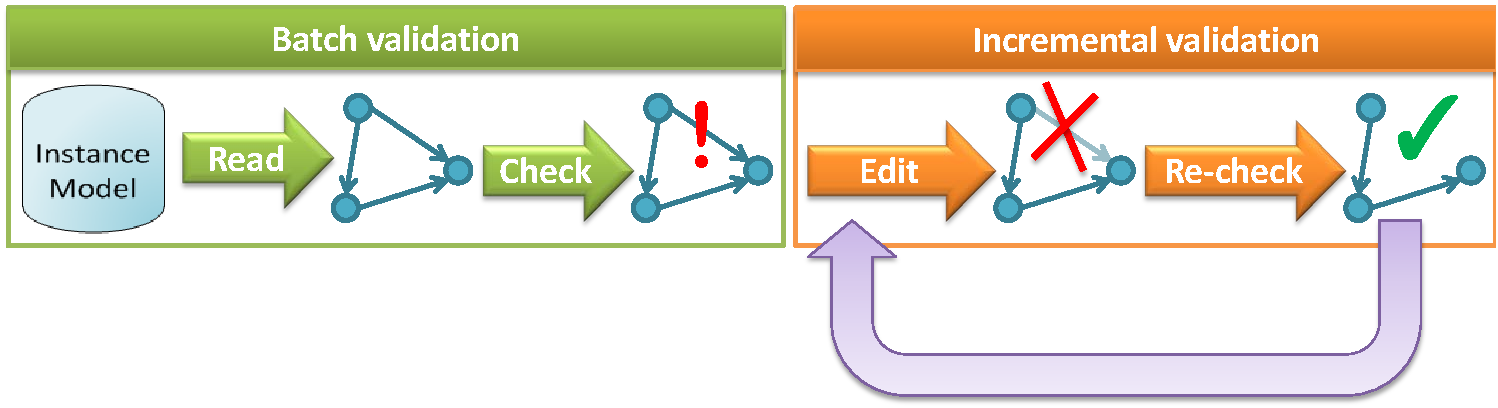
\includegraphics[scale=0.5]{figures/phases}
	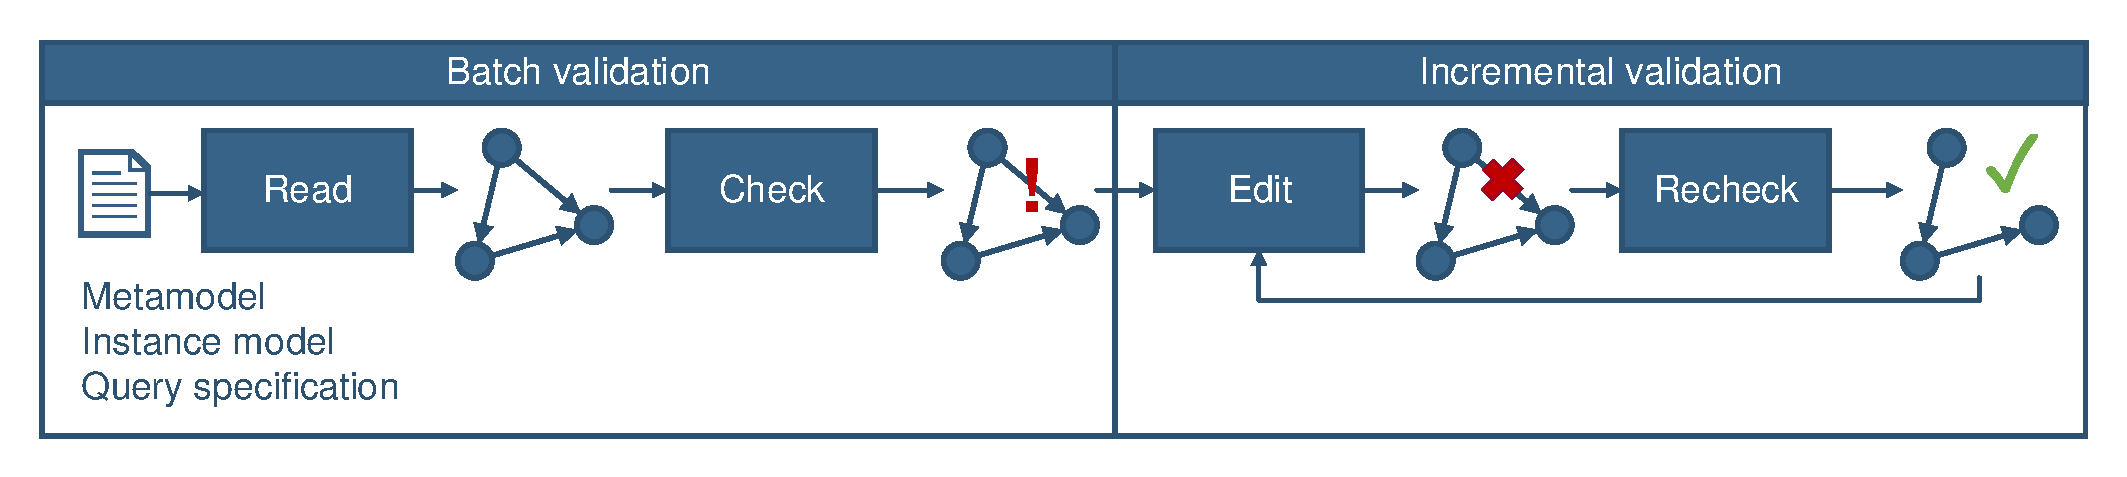
\includegraphics[width=\textwidth]{figures/trainbenchmark-sequence}
	\caption{The phases of the benchmark.}
	\label{fig:phases}
\end{figure}

To measure performance for re-validating a model after modifications, four benchmark \concept{phases} were defined, as illustrated in \figref{fig:phases}.
\begin{enumerate}
 
 \item During the \concept{read} phase, the previously generated instance model and validation query are loaded from hard drive to memory. This includes the parsing of the input as well as initializing data structures of the tool.
 
 \item In the \concept{check} phase, the instance model is queried to identify invalid elements. This can be as simple as reading the results from cache, or the model can be traversed based on some index. By the end of this phase, erroneous objects need to made available in a collection for further processing.
 
 \item In the \concept{edit} phase, the model is changed to simulate effects (and measure performance) of model modifying operations. At the beginning of this phase ``query-like'' functions are used to gather elements to be modified, however this time is excluded, and only the required time of model editing operations are recorded in this phase. (As query performance is measured in the check phases.)
 
 \item The re-validation of the model is carried out in the \concept{re-check} phase similarly to the \emph{check} phase.
\end{enumerate}

\subsection{Use Case Scenarios of the Benchmark}
\label{sec:scenarios}

Paper~\cite{icgt08-bhrv} analyzes performance of algorithms used for graph
pattern query evaluation and identifies two use cases where efficient
\emph{incremental model validation} is required. The batch part of our benchmark
consists of the execution of the read and first check phases. Inspired by paper
\cite{icgt08-bhrv}, three \concept{scenarios} were defined to measure different
use cases:
\begin{itemize}
  
  \item \concept{Batch validation scenario} (\textsf{Batch}):
  In this scenario the model is \emph{read} in one batch from storage, than a model validation is carried out by executing the query in the check phase. Such use case is performed when a model editor is opened and initial validations are issued by the designer. 
  
  \item \concept{Automated model repair scenario} (\textsf{Repair}):
  The automated model repair scenario extends the batch validation scenario by differential model modification and re-checking phases. In the edit phase, the model is repaired, based on the erroneous objects identified during the batch validation. This is carried out by the tool itself performing mass edits automatically. Finally, the whole model is re-checked, and remaining or newly introduced errors are reported. 
  
  Efficient execution of such a use case is necessary during refactoring, incremental code generation, or when a model is transformed from a source language to a target language by a model transformation program, using model synchronisation.
  
  \item \concept{User model editing scenario} (\textsf{User}):
  The user model editing scenario extends the batch validation scenario by differential model modification and re-checking phases. After the batch validation a small model manipulation step is performed (e.g.\ a reference is deleted), which is immediately followed by re-validation to get instantaneous feedback.  In this scenario such small edit and re-check phases are executed in sequence.
  
  Such scenario occurs when someone uses a typical UML editor (for designing software solutions), or a domain-specific editor where elements or relations are added one-by-one. These editors should detect design errors quickly and early in the development process to let engineers refine models and cut down debugging and error correction costs.
  
\end{itemize}


\subsection{Metamodel}
\label{sec:domain}

\begin{figure}[htb]
\begin{center}
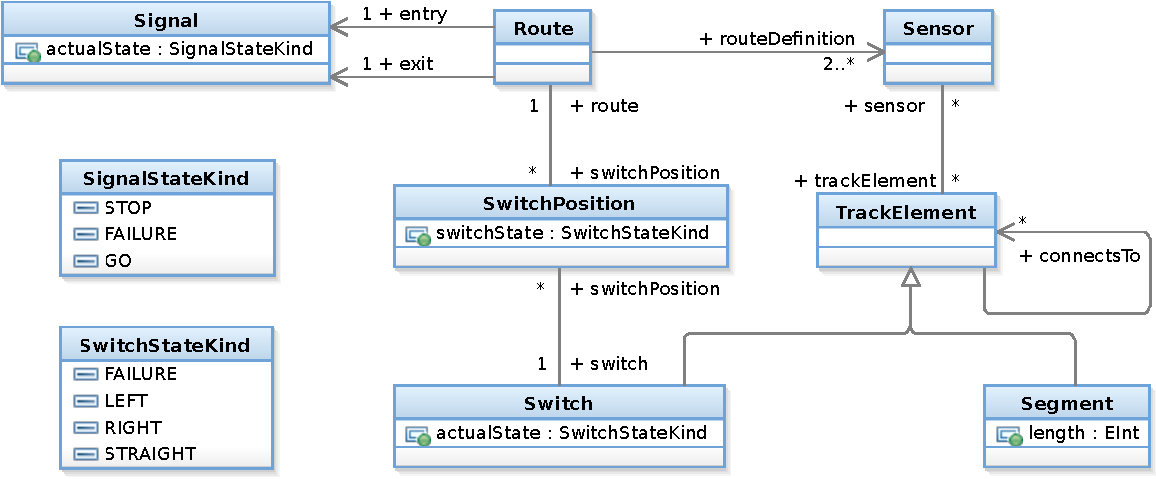
\includegraphics[width=1\columnwidth]{figures/TrainMM.pdf}
\caption{The railway metamodel used in the Train Benchmark.}
\label{fig:metamodel}
\end{center}
\end{figure}


The metamodel of the railway domain used in the Train Benchmark is depicted in \figref{fig:metamodel}. A train \textsf{route} can be defined by a set of \textsf{sensors}. Sensors are associated with \textsf{track elements}: track \textsf{segment}s (with a specific length) or \textsf{switch}es. A route may have associated \textsf{switch positions} which describe the required state of a switch belonging to the route. Different route definitions can specify different states for a specific switch.
 
\subsection{Queries}
\label{sec:queries}

In the validation and re-validation phases of the benchmark, the queries return the elements violating the well-formedness constraint defined by the test case. These constraints are first defined informally in plain text and then formalized using a query language suited for the benchmarked tool. As a result, the query must return a set of the invalid instance model elements' identifiers.
 
Two simple queries involving maximum 2 objects (\textsf{PosLength} and \textsf{SwitchSensor}) and two complex queries involving 4--8 objects and multiple join operations (\textsf{RouteSensor} and \textsf{SemaphoreNeighbor}) were defined. Simple queries are able to quickly distinguish efficient tools from inefficient ones, while complex queries are used to differentiate faster model query technologies.
 
In the following, we present the queries defined in the \tb{}. We describe the semantics and the goal of each query. We also show the associated graph pattern and relational algebra query.

\subsubsection{Relational Schemas}

For formulating the queries in relational algebra we define the following relational schemas for representing the vertices (objects) in the graph (instance model).

\begin{itemize}
  \item $ \mathit{Route}\left(\mathit{id}\right) $
  \item $ \mathit{Sensor}\left(\mathit{id}, \mathit{Segment\_length}\right) $
  \item $ \mathit{Signal}\left(\mathit{id}\right) $
  \item $ \mathit{Switch}\left(\mathit{id}\right) $
  \item $ \mathit{SwitchPosition}\left(\mathit{id}\right) $
  \item $ \mathit{TrackElement}\left(\mathit{id}\right) $
\end{itemize}

The edges\footnote{also called relationships or references in various implementations} are represented with the following relational schemas:

\begin{itemize}
  \item $ \mathit{entry}\left(\mathit{Route}, \mathit{Signal}\right) $
  \item $ \mathit{exit}\left(\mathit{Route}, \mathit{Signal}\right) $
  \item $ \mathit{switchPosition}\left(\mathit{Route}, \mathit{SwitchPosition}\right) $
  \item $ \mathit{routeDefinition}\left(\mathit{Route}, \mathit{Sensor}\right) $
  \item $ \mathit{switch}\left(\mathit{SwitchPosition}, \mathit{Switch}\right) $
  \item $ \mathit{sensor}\left(\mathit{Switch}, \mathit{Sensor}\right) $
  \item $ \mathit{connectsTo}\left(\mathit{TrackElement}, \mathit{TrackElement}\right) $
\end{itemize}

\subsubsection{Graph Patterns}

In the following, we represent the graph pattern representation for the violation of each well-formedness constraint. Opaque blue rectangles and dashed arrows mark positive constraints, while red rectangles and arrows represent negative application conditions (NACs). The result of the query (also referred as the \emph{match set}) is marked with transparent blue rectangles. Additional constraints (e.g.\ arithmetic comparisons) are shown in the figure in text.

%%%%%%%%%%%%%%%%%%%%%%%%%%%%%%%%%%%%%%%%%%%%%%%%%%%%%%%%%%%%%%%%%%%%%%%%%%%%%%%

\subsubsection{PosLength}

\paragraph{Description.} The \textsf{PosLength} well-formedness constraint requires that a segment must have positive length. Therefore, the query (\figref{fig:pattern-poslength}) checks for segments with a length less than or equal to zero. The SPARQL representation of the query is shown in \lstref{lst:poslength-sparql}.

\paragraph{Goal.} The query checks whether an object has an attribute. If it does, the value is checked. Checking attributes is a real world use case, even if a very simple one. Note that simple string checking is also measured in the Berlin SPARQL Benchmark~\cite{BSBM} and it concludes that for most tools the string comparison algorithm dominates the query time.

\begin{figure}[htb]
\centering
\begin{minipage}{0.5\textwidth}
  { \alignListing
    \sourceSPARQL{figures/queries/PosLength.sparql}}
  \caption{\textsf{PosLength} query in SPARQL.}
  \label{lst:poslength-sparql}
\end{minipage}
\end{figure}

\begin{figure}[htb]
		\centering
		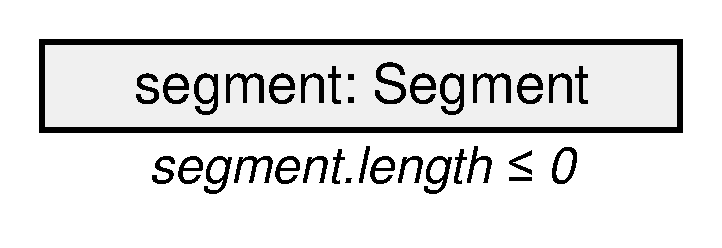
\includegraphics[scale=0.4]{figures/pattern-poslength}
		\caption{The \textsf{PosLength} pattern.}
		\label{fig:pattern-poslength}
\end{figure}

\paragraph{Relational algebraic form.} The \textsf{PosLength} query can be formalized in relational algebra as:

$$ \pi_{\mathit{id}} \left( \sigma_{\mathit{length} \leq 0} \left( \mathit{Sensor} \right) \right) $$

%%%%%%%%%%%%%%%%%%%%%%%%%%%%%%%%%%%%%%%%%%%%%%%%%%%%%%%%%%%%%%%%%%%%%%%%%%%%%%%
\subsubsection{RouteSensor}

\paragraph{Description.} The \textsf{RouteSensor} well-formedness constraint requires that all sensors that are associated with a switch that belongs to a route must also be associated directly with the same route. Therefore, the query (\figref{fig:pattern-routesensor}) looks for sensors that are connected to a switch, but the sensor and the switch are not connected to the same route. The SPARQL representation of the query is shown in \lstref{lst:routesensor-sparql-nac}.

\paragraph{Goal.} This pattern checks for the absence of circles, so the efficiency of the join and the antijoin operations is tested.

\begin{figure}[htb]
\centering
\begin{minipage}{0.6\textwidth}
  { \alignListing
    \sourceSPARQL{figures/queries/RouteSensor_neg.sparql}}
  \caption{The \textsf{RouteSensor} query in SPARQL 1.1.}
  \label{lst:routesensor-sparql-nac}
\end{minipage}
\end{figure}

\paragraph{Remark.} Note that the negative application condition (NAC) part (\texttt{FILTER NOT EXISTS}) is a SPARQL 1.1 feature. In SPARQL 1.0, we have to use the approach shown in \lstref{lst:routesensor-sparql-nac10}.

\begin{figure}[htb]
\centering
\begin{minipage}{0.6\textwidth}
  { \alignListing
    \sourceSPARQL{figures/queries/RouteSensor.sparql}}
  \caption{The NAC of the \textsf{RouteSensor} pattern in SPARQL 1.0.}
  \label{lst:routesensor-sparql-nac10}
\end{minipage}
\end{figure}

\begin{figure}[htb]
		\centering
		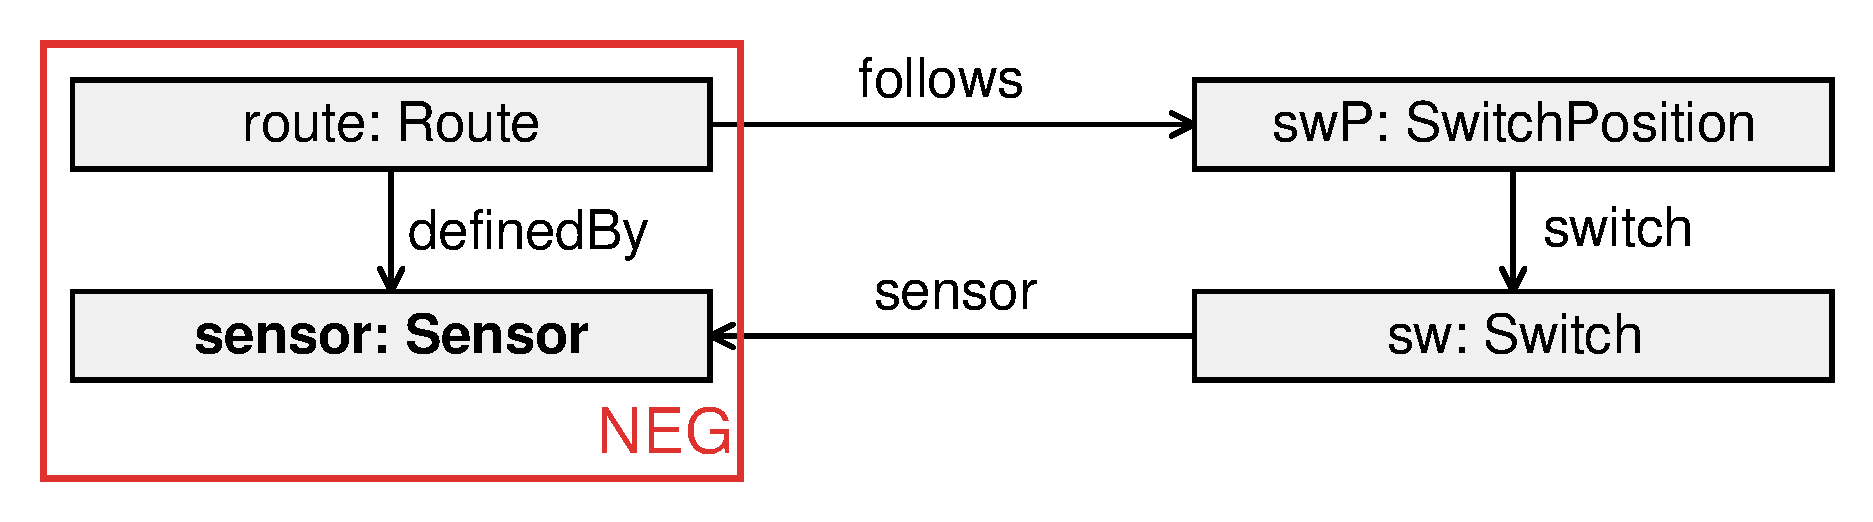
\includegraphics[scale=0.4]{figures/pattern-routesensor}
		\caption{The \textsf{RouteSensor} pattern.}
		\label{fig:pattern-routesensor}
\end{figure}

\paragraph{Relational algebraic form.}  The \textsf{RouteSensor} query can be formalized in relational algebra as:

\[
\pi_{\mathit{Route}} \big( \mathit{switchPosition} \naturaljoin \mathit{switch} \naturaljoin \mathit{sensor} \antijoin \mathit{routeDefinition} \big)
\]

%%%%%%%%%%%%%%%%%%%%%%%%%%%%%%%%%%%%%%%%%%%%%%%%%%%%%%%%%%%%%%%%%%%%%%%%%%%%%%%
\subsubsection{SemaphoreNeighbor}

\paragraph{Description.} The \textsf{SemaphoreNeighbor} well-formedness constraint requires that the routes that are connected through sensors and track elements have to belong to the same signal. Therefore, the query (\figref{fig:pattern-semaphoreneighbor}) checks for routes which have an exit signal and a sensor connected to another sensor (which is in a definition of another route) by two track elements, but there is no other route that connects the same signal and the other sensor. The SPARQL representation of the query is shown in \lstref{lst:semaphoreneighbor-sparql}.

\paragraph{Goal.} This pattern checks for the absence of circles, so the efficiency of the join operation is tested. One-way navigable references are also present in the constraint, so the efficient evaluation of these are also tested. Subsumption inference is required, as the two track elements can be switches or segments.

\begin{figure}[htb]
\centering
\begin{minipage}{0.6\textwidth}
  { \alignListing
    \sourceSPARQL{figures/queries/SemaphoreNeighbor.sparql}}
  \caption{The \textsf{SemaphoreNeighbor} query in SPARQL.}
  \label{lst:semaphoreneighbor-sparql}
\end{minipage}
\end{figure}

\begin{figure}[htb]
		\centering
		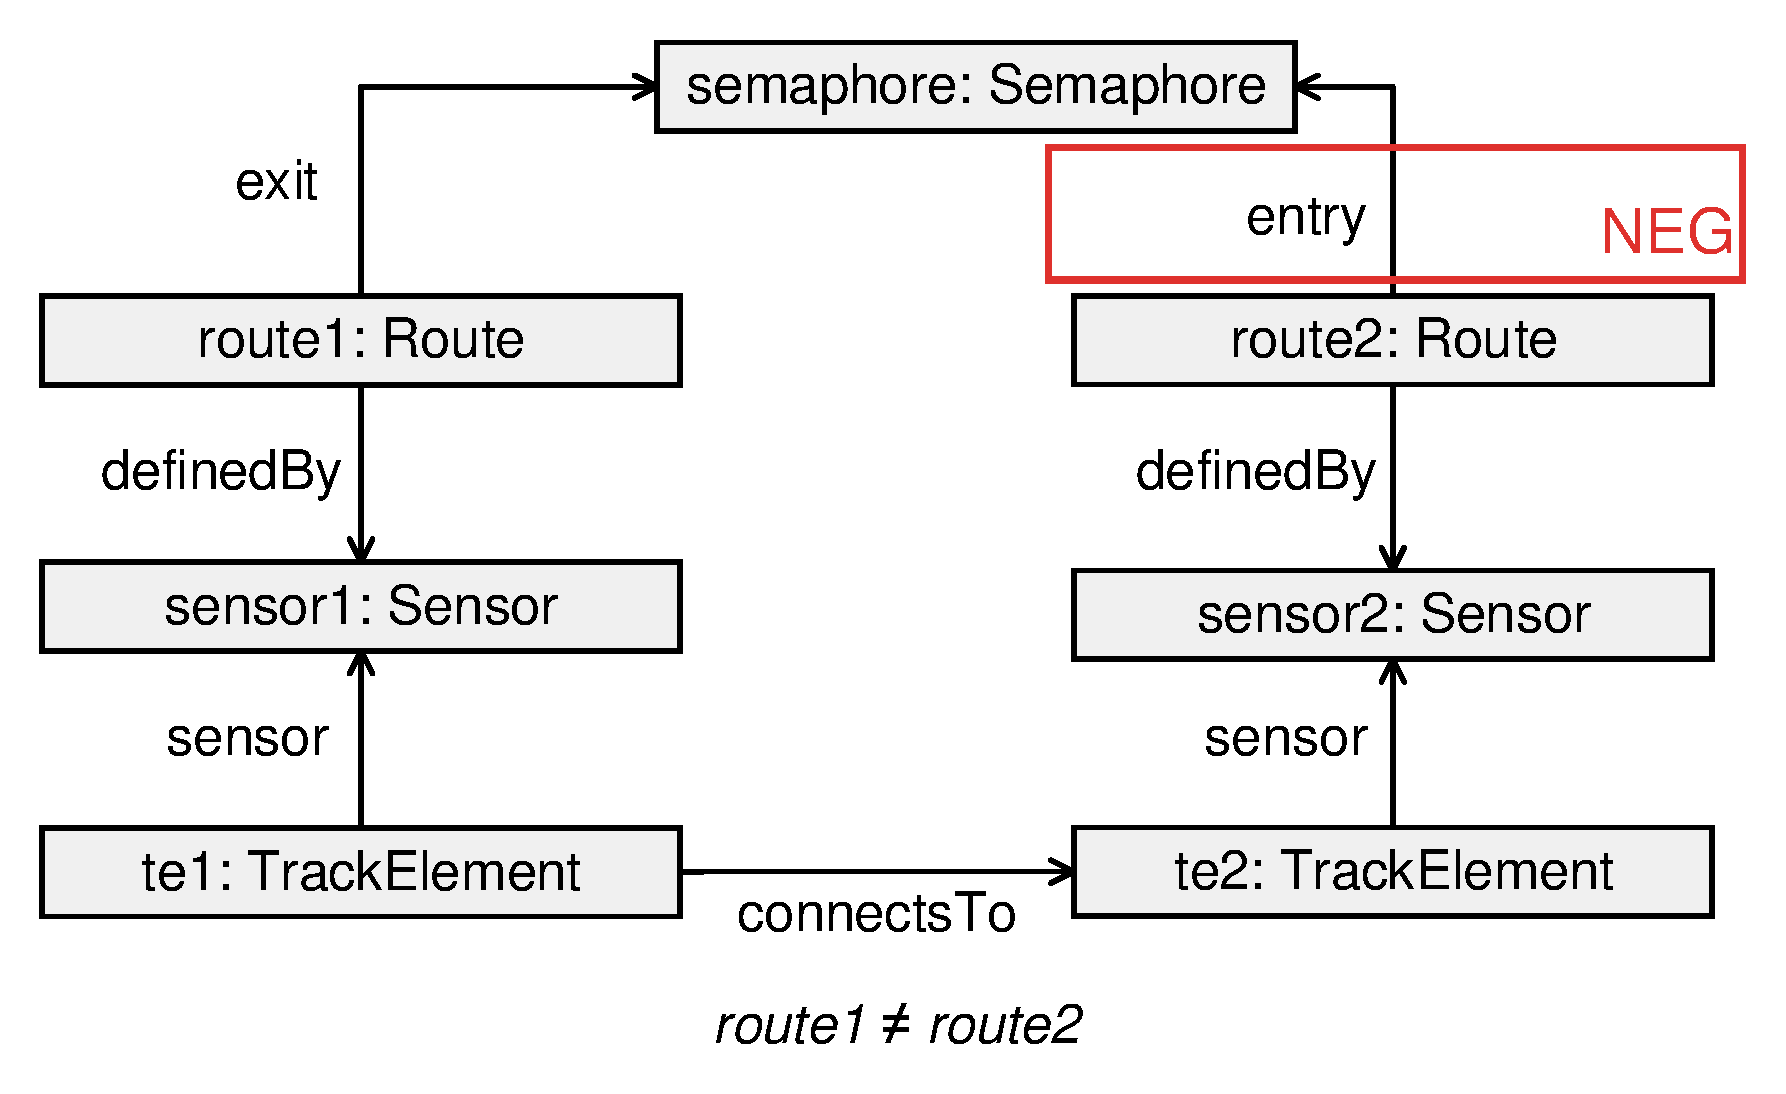
\includegraphics[scale=0.4]{figures/pattern-semaphoreneighbor}
		\caption{The \textsf{SemaphoreNeighbor} pattern.}
		\label{fig:pattern-semaphoreneighbor}
\end{figure}

\paragraph{Relational algebraic form.} The \textsf{SemaphoreNeighbor} query can be formalized in relational algebra as:

\begin{align*}
& \pi_{\mathit{entry.Route}} \big( \sigma_{\mathit{entry.Route} \neq \mathit{routeDefinition_2.Route}} \big( \\
& \quad \mathit{entry} \naturaljoin \mathit{routeDefinition_1} \naturaljoin \mathit{sensor_1} \naturaljoin \\
& \quad \mathit{connectsTo} \naturaljoin \mathit{sensor_2} \naturaljoin \mathit{routeDefinition_2} \antijoin \\
& \quad \left( \mathit{exit} \naturaljoin \mathit{routeDefinition_3} \right) \\
& \big) \big)
\end{align*}

%%%%%%%%%%%%%%%%%%%%%%%%%%%%%%%%%%%%%%%%%%%%%%%%%%%%%%%%%%%%%%%%%%%%%%%%%%%%%%%
\subsubsection{SwitchSensor}

\paragraph{Description.} The \textsf{SwitchSensor} well-formedness constraint requires that every switch must have at least one sensor connected to it. Therefore, the query (\figref{fig:pattern-switchsensor}) checks for switches that have no sensors associated with them. The SPARQL representation of the query is shown in \lstref{lst:switchsensor-sparql}.

\paragraph{Goal.} This query checks whether an object is connected to a relation. This pattern is common in more complex queries, e.g.\ it is used in the \textsf{RouteSensor} and the \textsf{SemaphoreNeighbor} queries.

\begin{figure}[htb]
\centering
\begin{minipage}{0.6\textwidth}
  { \alignListing
    \sourceSPARQL{figures/queries/SwitchSensor_neg.sparql}}
  \caption{The \textsf{SwitchSensor} query in SPARQL.}
  \label{lst:switchsensor-sparql}
\end{minipage}
\end{figure}


\begin{figure}[htb]
	\centering
	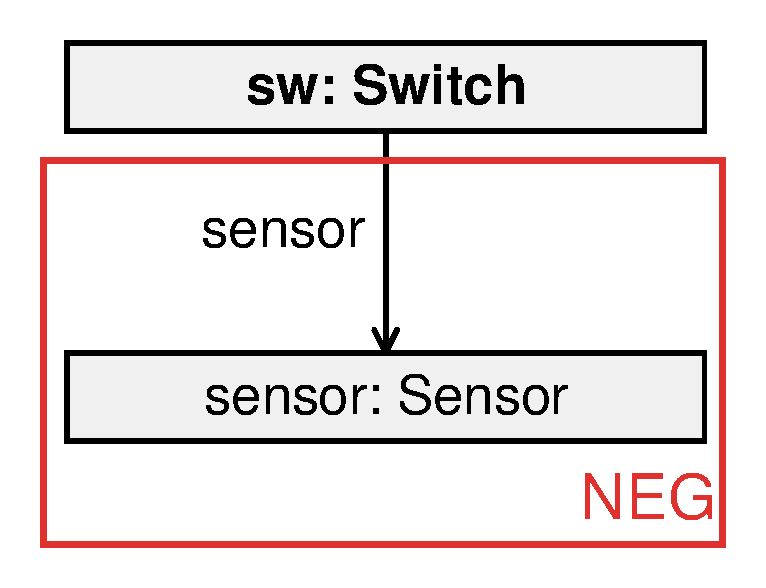
\includegraphics[scale=0.4]{figures/pattern-switchsensor}
	\caption{The \textsf{SwitchSensor} pattern.}
	\label{fig:pattern-switchsensor}
\end{figure}

\paragraph{Relational algebraic form.} The \textsf{SwitchSensor} query can be formalized in relational algebra as:

$$ \mathit{Switch} \antijoin \mathit{Sensor} $$


\subsection{Transformations}
\label{sec:transformatios}

In the \emph{edit} phase the model is modified to change the result set returned in the succeeding re-check phase.

The Train Benchmark defines model transformations for each query. The transformations are also represented as graph transformations. The insertions are shown in green with a \guillemotleft{}new\guillemotright{} caption, while deletions are marked with a red cross and a \guillemotleft{}del\guillemotright{} caption. In general, the goal of these transformations is to remove a subset of the invalid elements from the model.

\begin{table}[htb]
	\centering
	\scriptsize
	\begin{tabular}{r|r|r|r|r|r|r|r|r|r|}
	\cline{2-9}
	& \multicolumn{4}{ c| }{\bf User (modify = 10)} & \multicolumn{4}{ c| }{\bf Repair (modify = Res1 × 10\%)} \\ \hline
	\multicolumn{1}{ |r| }{\bf\#Objects} & \bf \#Sensors & \bf Result1 & \bf Modify RS & \bf Result2 & \bf \#Sensors & \bf Result1 & \bf Modify RS & \bf Result2 \\ \hline
	\multicolumn{1}{ |r| }{6032}         & 928 & 19 & 10 & 29 & 967 & 94 & 9 & 85 \\ \hline
	\multicolumn{1}{ |r| }{11710}        & 1804 & 41 & 10 & 51 & 1936 & 193 & 19 & 174 \\ \hline
	\multicolumn{1}{ |r| }{23180}        & 3575 & 68 & 10 & 76 & 3545 & 348 & 34 & 314 \\ \hline
	\multicolumn{1}{ |r| }{46728}        & 7210 & 140 & 10 & 150 & 6691 & 642 & 64 & 578 \\ \hline
	\multicolumn{1}{ |r| }{87396}        & 13465 & 264 & 10 & 274 & 13650 & 1301 & 130 & 1171 \\ \hline
	\multicolumn{1}{ |r| }{175754}       & 27074 & 510 & 10 & 520 & 27190 & 2606 & 260 & 2346 \\ \hline
	\multicolumn{1}{ |r| }{354762}       & 54653 & 1048 & 10 & 1058 & 55708 & 5324 & 532 & 4792 \\ \hline
	\multicolumn{1}{ |r| }{708770}       & 109185 & 2071 & 10 & 2081 & 110291 & 10623 & 1062 & 9561 \\ \hline
	\multicolumn{1}{ |r| }{1415954}      & 218140 & 4215 & 10 & 4224 & 219305 & 21097 & 2109 & 18988 \\ \hline
	\multicolumn{1}{ |r| }{2837336}      & 437089 & 8501 & 10 & 8510 & 437025 & 41762 & 4176 & 37586 \\ \hline
	\end{tabular}
	\caption{Modification in the \textsf{RouteSensor} test case.}
	\label{tbl:modify_RouteSensor}
\end{table}

\autoref{tbl:modify_RouteSensor}. shows the instance model characteristics and the effect of the modify phase in the \textsf{RouteSensor} case. The first column counts the number of instance model elements. The second and the fifth column show the number of Sensors in the model. The two scenarios process different instance models and modify them differently:

\begin{itemize}
	\item In the \emph{User scenario} (where a developer is assumed to sit in front of an editor) the initial number of constraint violating elements are low (0.3\% of model elements for the \textsf{RouteSensor} case), so it can be understood and resolved by a user using the editor.
	
	During the modification the user always performs 10 random edits (fixed low constant) which \emph{increase} the number of erroneous elements. These edit operations modify only some elements of the model and do not add or remove modules containing multiple instance model elements.

	\item In the \emph{Repair scenario} the initial number of errors is higher (1.5\% of objects for the \textsf{RouteSensor} case). This scenario models the case when these errors are (partially) processed by a model transformation program automatically.

	In the edit phase the program modifies 10\% of the elements of the result set retrieved from the batch query. These modifications always correct an invalid element in the model, so the number of invalid elements \emph{decreases} (see \autoref{tbl:modify_type}).

\end{itemize}


\autoref{tbl:modify_type}. displays the effect of model changes to the result set size and the type of edit operations (add, update, delete).

\begin{table}[h]
	\centering
	\begin{tabular}{l|l|l|l|l|l|}
	\cline{2-5}
	& \multicolumn{2}{ c| }{\bf User} & \multicolumn{2}{ c| }{\bf Repair} \\ \cline{2-5}
	& \bf Modification type & \bf RSS change & \bf Modification type & \bf RSS change \\ \hline
	\multicolumn{1}{ |l| }{\bf PosLength}      & Update & Increase & Update & Decrease \\ \hline
	\multicolumn{1}{ |l| }{\bf SwitchSensor}   & Delete & Increase & Add    & Decrease \\ \hline
	\multicolumn{1}{ |l| }{\bf RouteSensor}    & Delete & Increase & Delete & Decrease \\ \hline
	\multicolumn{1}{ |l| }{\bf SemaphoreNeighbor} & Update & Increase & Update & Decrease \\ \hline
	\end{tabular}
	\caption{Modification type for the queries.}
	\label{tbl:modify_type}
\end{table}

\begin{figure}
        \centering
        \begin{subfigure}[b]{0.4\textwidth}
        		\centering
                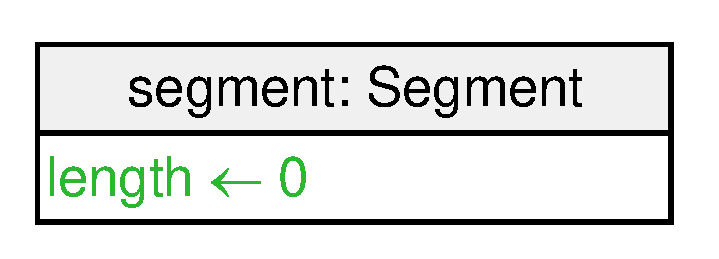
\includegraphics[scale=0.4]{figures/transformation-user-poslength}
                \caption{\textsf{PosLength}}
                \label{fig:transformation-user-poslength}
        \end{subfigure}%
        ~
        \begin{subfigure}[b]{0.6\textwidth}
                \centering
                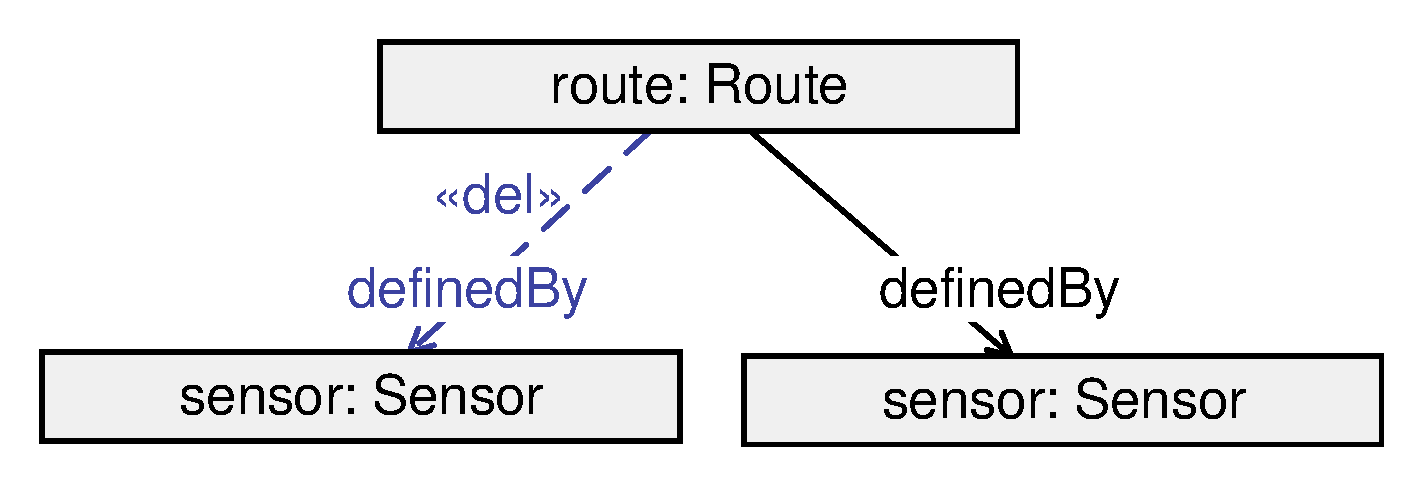
\includegraphics[scale=0.4]{figures/transformation-user-routesensor}
                \caption{\textsf{RouteSensor}}
                \label{fig:transformation-user-routesensor}
        \end{subfigure}
        ~
        \begin{subfigure}[b]{0.4\textwidth}
                \centering
                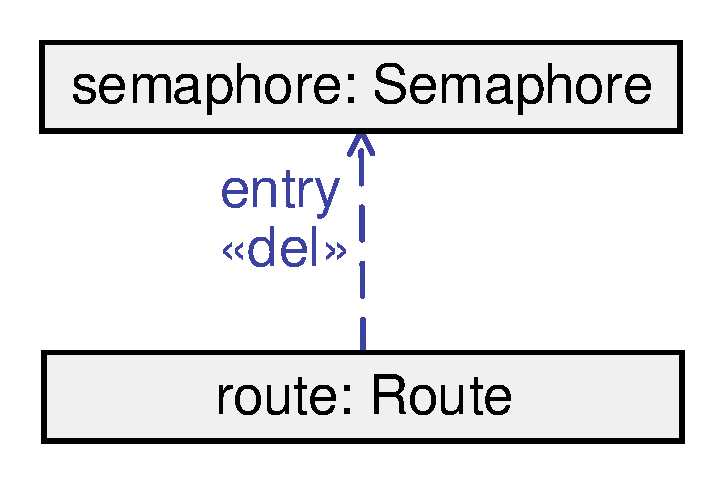
\includegraphics[scale=0.4]{figures/transformation-user-semaphoreneighbor}
                \caption{\textsf{SemaphoreNeighbor}}
                \label{fig:transformation-user-semaphoreneighbor}
        \end{subfigure}%
        ~
        \begin{subfigure}[b]{0.6\textwidth}
                \centering
                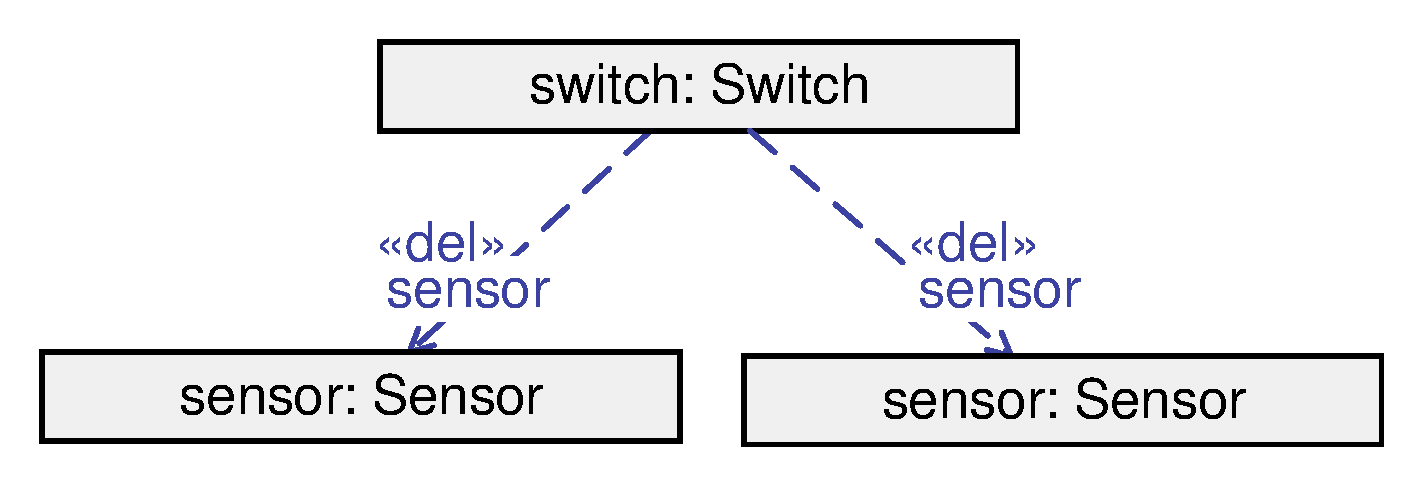
\includegraphics[scale=0.4]{figures/transformation-user-switchsensor}
                \caption{\textsf{SwitchSensor}}
                \label{fig:transformation-user-switchsensor}
        \end{subfigure}
        \caption{Transformations in the User scenario.}
        \label{fig:transformations-repair}
\end{figure}


The modifications in more detail:
\begin{itemize}
  \item \emph{User scenario:} in this case elements to be edited are selected from the whole instance model, i.e.\ they may be valid or invalid. 
  \begin{itemize}
    
    \item \emph{PosLength:} Randomly selected \emph{segments'} \emph{length} attribute is updated to 0, which means that an error is injected (\figref{fig:transformation-user-poslength}).\footnote{In EMF this means that an \texttt{int} attribute is set (updated), while in other representations (e.g.\ RDF databases) first the assertion about the old value is removed and the assertion stating the new value of the length is inserted.}
    
    \item \emph{RouteSensor:} The \emph{routeDefinition} edges between the randomly selected \emph{routes} and their \emph{first} connected \emph{sensor} are removed (at most one edge for each route, see~\figref{fig:transformation-user-routesensor}).
    
    \item \emph{SemaphoreNeighbor:} Errors are introduced by disconnecting the \emph{entry} edge of the selected \emph{routes} (\figref{fig:transformation-user-semaphoreneighbor}). (According to the metamodel, a \emph{route} may only have 0 or 1 \emph{entry} edges).

    \item \emph{SwitchSensor:} Errors are injected by randomly selecting \emph{switches} and deleting all their edges to \emph{sensors}. If the chosen \emph{switch} was invalid, it did not have such an edge, so no edges are deleted and the \emph{switch} stays invalid. If the chosen \emph{switch} was valid, it will become invalid (\figref{fig:transformation-user-switchsensor}).
        
\end{itemize}
  
  
\begin{figure}
        \centering
        \begin{subfigure}[b]{\textwidth}
        		\centering
                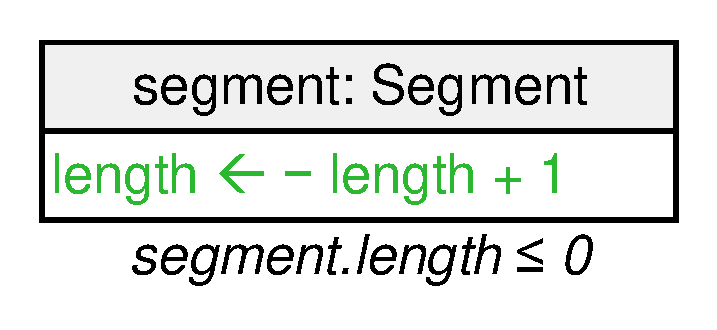
\includegraphics[scale=0.4]{figures/transformation-repair-poslength}
                \caption{\textsf{PosLength}}
                \label{fig:transformation-repair-poslength}
        \end{subfigure}
        ~
        \begin{subfigure}[b]{\textwidth}
                \centering
                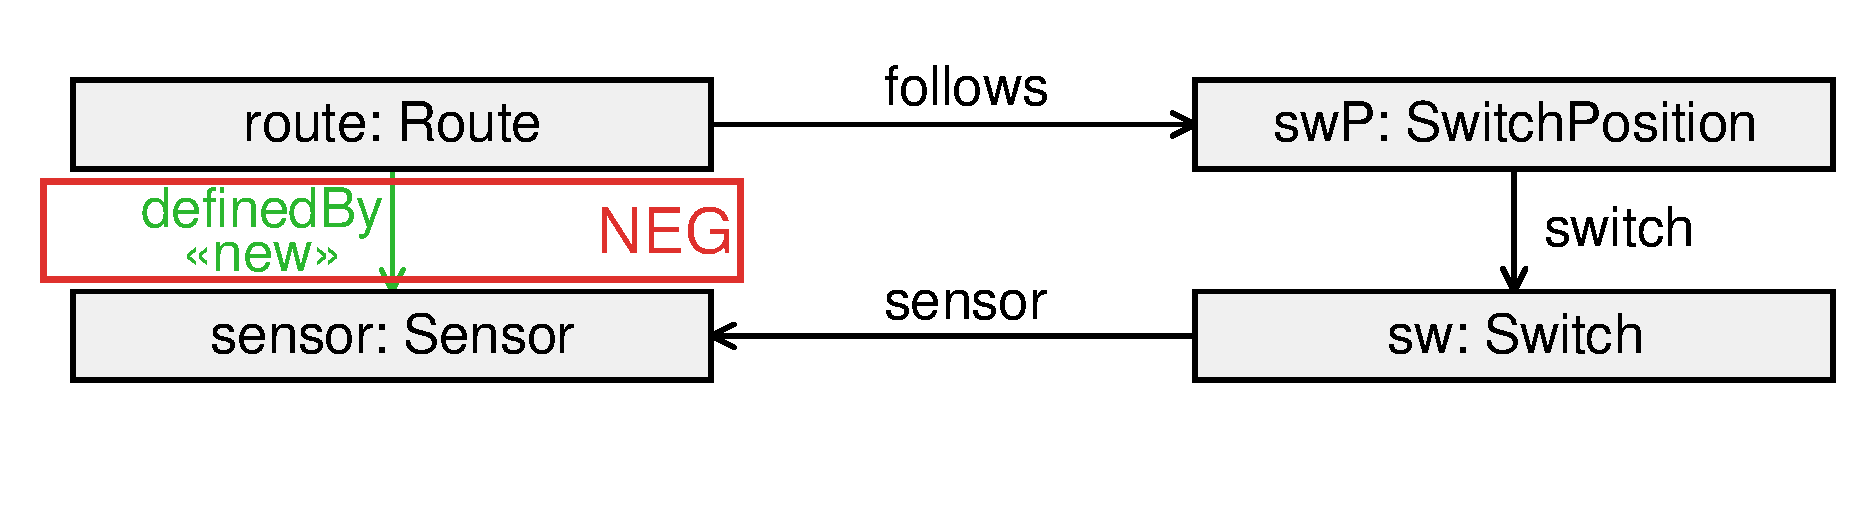
\includegraphics[scale=0.4]{figures/transformation-repair-routesensor}
                \caption{\textsf{RouteSensor}}
                \label{fig:transformation-repair-routesensor}
        \end{subfigure}
        ~
        \begin{subfigure}[b]{\textwidth}
                \centering
                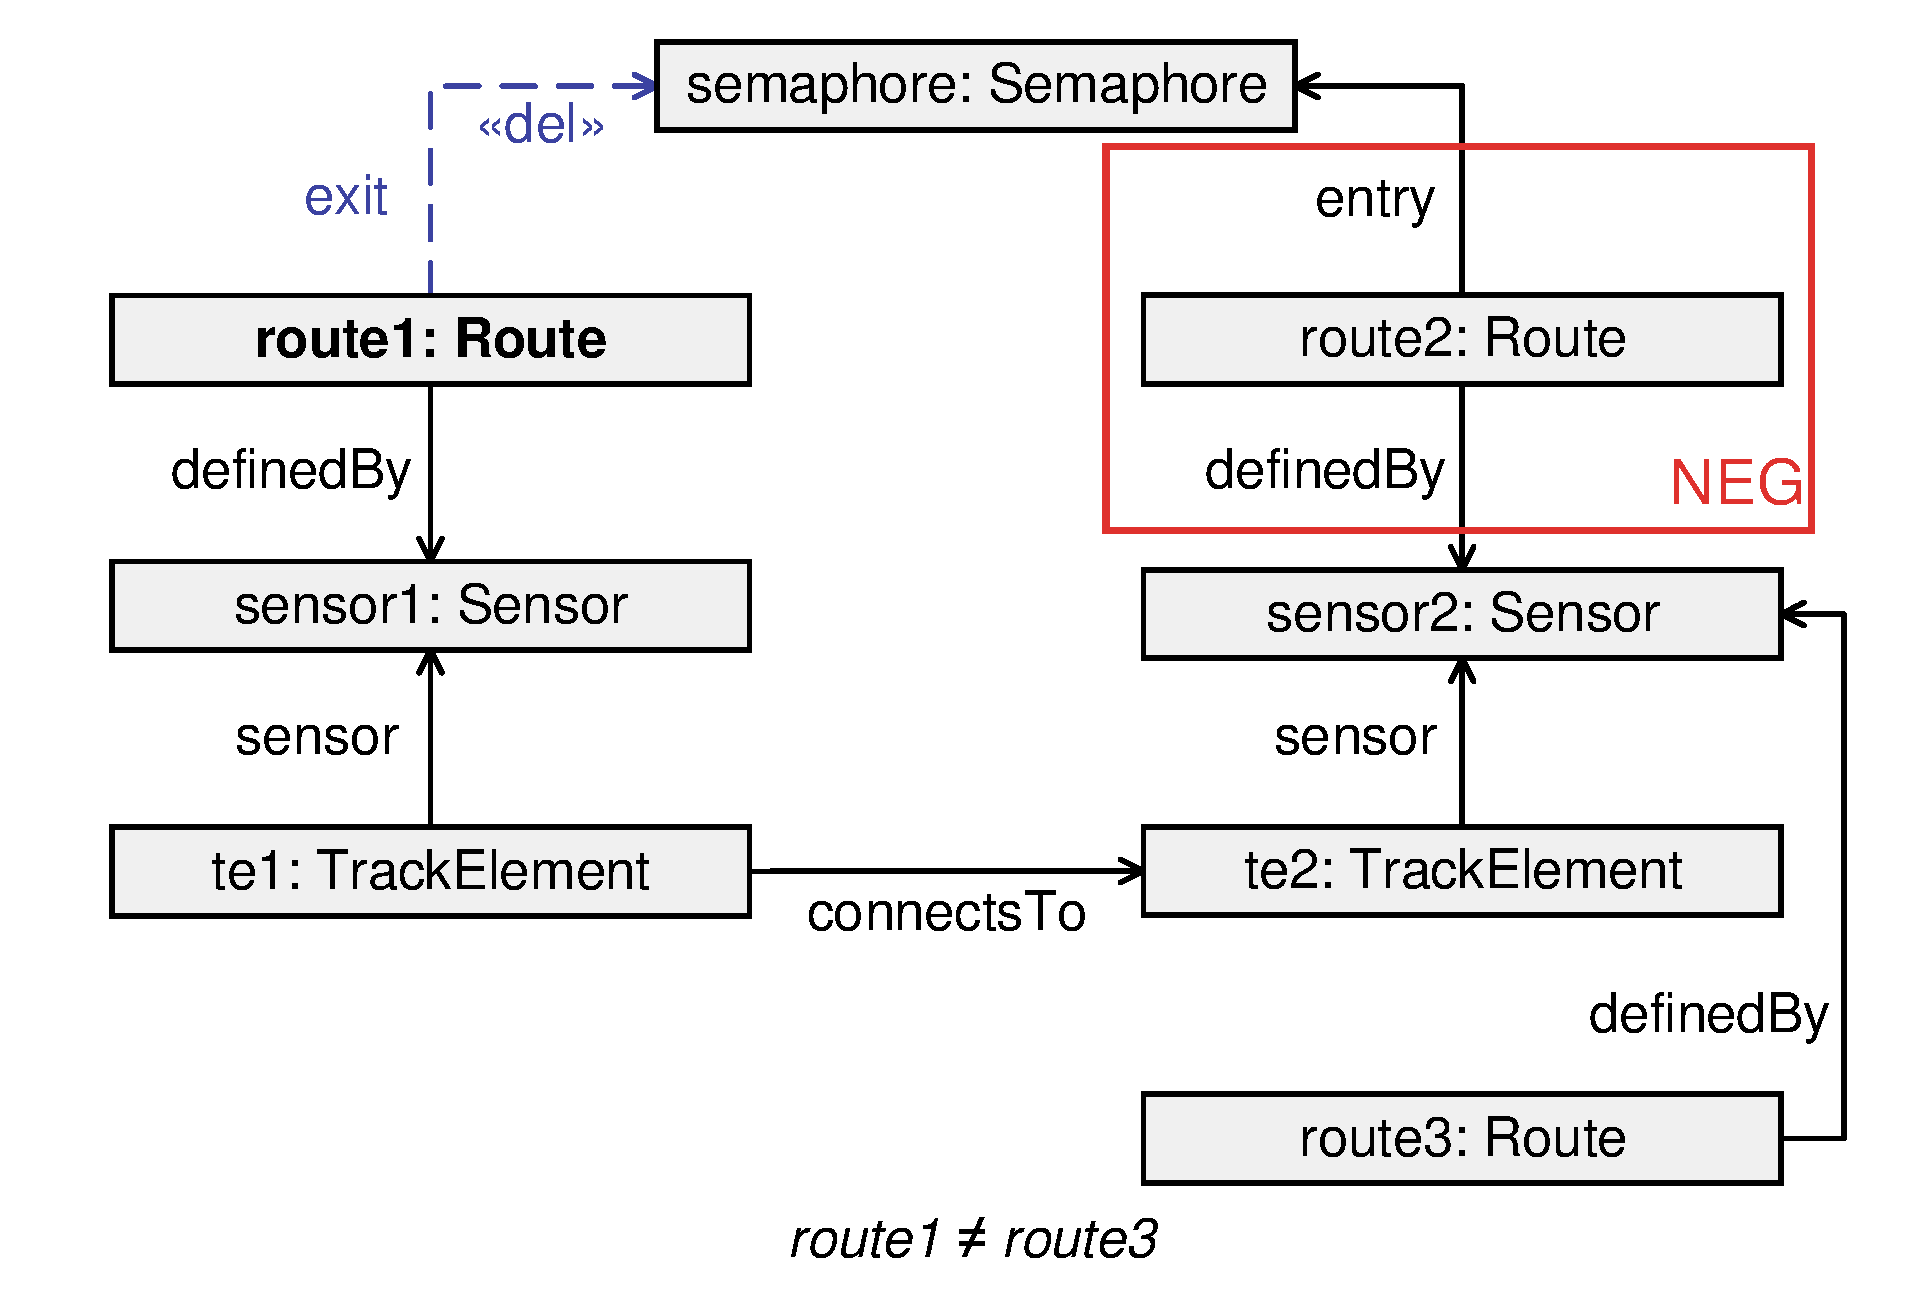
\includegraphics[scale=0.4]{figures/transformation-repair-semaphoreneighbor}
                \caption{\textsf{SemaphoreNeighbor}}
                \label{fig:transformation-repair-semaphoreneighbor}
        \end{subfigure}
        ~
        \begin{subfigure}[b]{\textwidth}
                \centering
                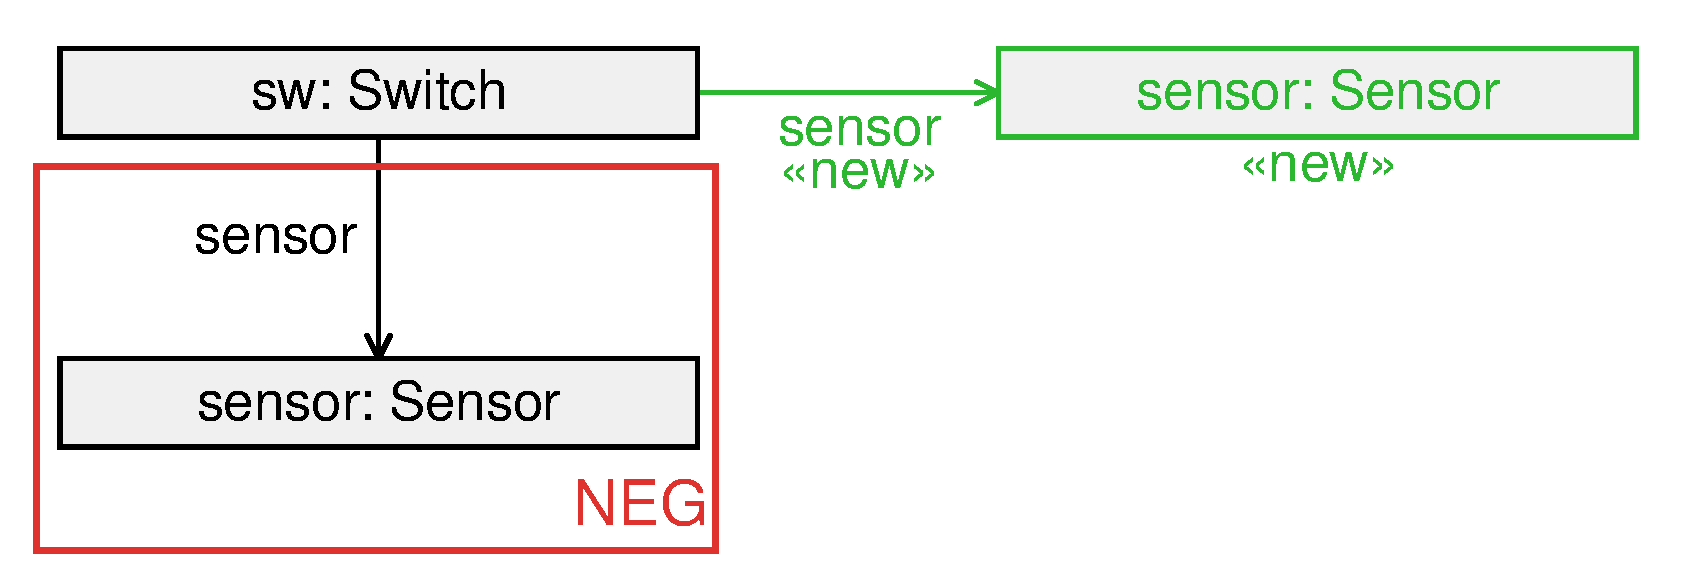
\includegraphics[scale=0.4]{figures/transformation-repair-switchsensor}
                \caption{\textsf{SwitchSensor}}
                \label{fig:transformation-repair-switchsensor}
        \end{subfigure}
        \caption{Transformations in the Repair scenario.}
        \label{fig:transformations-repair}
\end{figure}
  
  \item \emph{Repair scenario:} in this case elements to be edited are selected from the result of the previous query. The transformations provide quick fix-like repair operations.
  \begin{itemize}
    
    \item \emph{PosLength:} Random elements are selected from the set of invalid \emph{segments} and their values are updated to $- \mathit{oldValue} + 1$ (\figref{fig:transformation-repair-poslength}).
    
    \item \emph{RouteSensor:} Randomly selected invalid \emph{sensors} are disconnected from the \emph{switch}, which means that the constraint will no longer apply (\figref{fig:transformation-repair-routesensor}).
    
    \item  \emph{SemaphoreNeighbor:} Disconnect \emph{exit} references of randomly selected invalid \emph{routes}, resulting in a structure where the constraint must not hold for the actual route (\figref{fig:transformation-repair-semaphoreneighbor}).
        
    \item \emph{SwitchSensor:} Random elements are selected from the set of invalid \emph{switches} and are connected to newly created \emph{sensors}.
    
    In EMF this means the creation of a new Sensor which is added to the switch and also to the root container object. In ontology the triples asserting the connection between the new Sensor and the Switch, as well as its type are inserted into the knowledge base (\figref{fig:transformation-repair-switchsensor}).
    
  \end{itemize}
\end{itemize}


\subsection{Instance Model Generation}
\label{sec:instanceGeneration}

In the first phase of the benchmark, a previously generated \concept{instance model} is loaded from the file system. These models are systematically generated based on the metamodel and on the model queries. Randomized instance model fragments are generated and connected to each other. The generation process takes care of controlling the number of matches for all model queries.

To break symmetry, the exact number of elements and cardinalities are randomized. This brings artificially generated models \emph{closer to real world instances}, and \emph{prevents query tools from this kind of efficient storing} of instance models. During the generation of the railway system model, errors are injected at random positions. The initial number of constraint violating elements that are low (below one percent of the total number of elements), and are deterministically placed, thanks to \emph{pseudorandom} generation. These errors have to be found in the check phase of the benchmark, and can be corrected during the edit phase.

\begin{figure}[htb]
\begin{center}
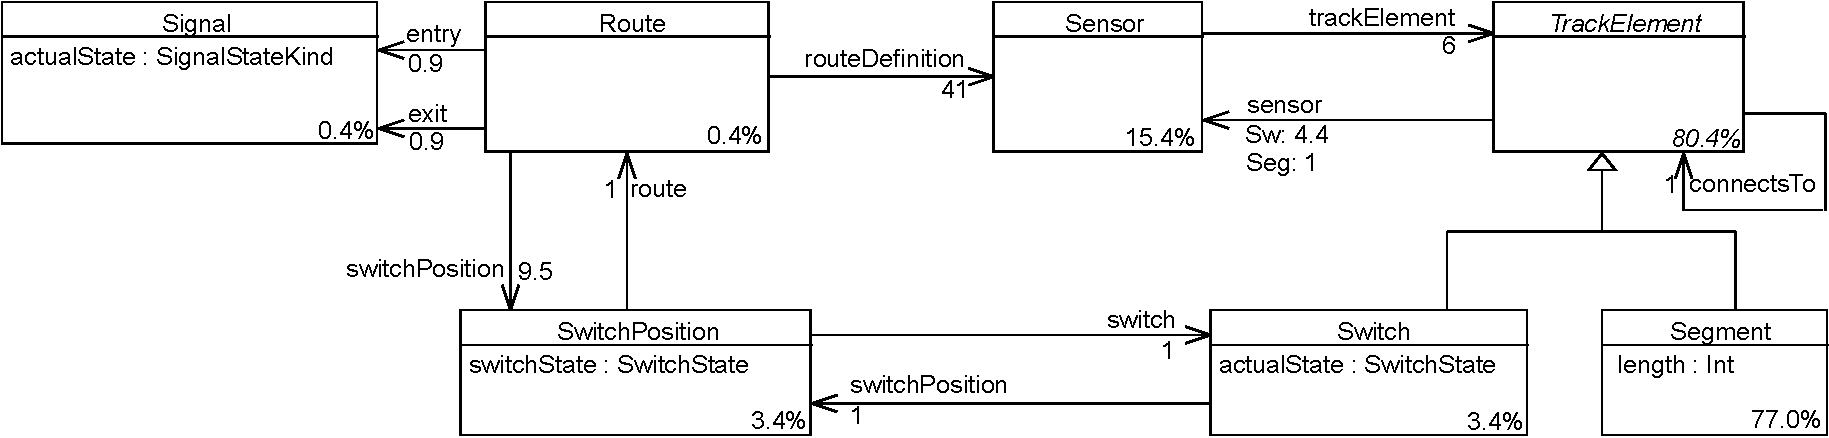
\includegraphics[width=\textwidth]{figures/instance/TrainMMb.pdf}
\caption{The railway metamodel and instance model characteristics.}
\label{fig:metamodel-instance-characteristics}
\end{center}
\end{figure}

To show some characteristics of the generated instance models, the distribution of the object types and the average number of edges for each object are presented in \autoref{fig:metamodel}. In the case of classes the percentage of instances is shown: e.g.\ 3.4\% of the model elements are instance of the class \emph{Switch}, 77.0\% are \emph{Segment}s, thus 80.4\% are \emph{TrackElement}s. The average number of the given relation for an instance is displayed for associations: e.g.\ there are 9.5 \emph{switchPosition} relations in average for every instance of the \emph{Route} class.
